\section{Impedance Variation vs Frequency}
Sampling data from between 6.3 MHz and 7.7 MHz, the length of the dipole was
set to be 48.457\% of wavelength $\lambda$ in order to acheive resonance.
Resonance is defined by the Antenna Impedance shown in Equation (\ref{eq:za}):
\begin{align}
  Z_A&=R_A+jX_A [\Omega]\label{eq:za}
\end{align}
Where if the reactance $X_A=0$, the antenna becomes resonant.
This meant that instead of the dipole being 20 meters long, it
would be in total only 19.38 meters long. This would be about 30.86 cm removed on each side of the
dipole.
\subsection{Demonstration of Resonance}
By decreasing the length of the antenna, the radiation resistance was lowered
such that $X_A=0$ when the frequency is 7 Mhz. This is shown in Figure~\ref{fig:impedance},
where the dotted line represents the reactance $X_A$ and the solid line is the
radiation resistance $R_A$. Since we are working under ideal free-space condtions,
there are no losses on the antenna, that is, $R_A=R_r$. Using FEKO, this value was
found to be $R_r \approx 75.65\Omega$. An approximation is available to confirm
the analysis conducted by FEKO. This is provided by Rutledge \cite{ER}, where a
dipole is expected to have $R_r$ around 73$\Omega$.

\begin{figure}[h!]
  \centering
  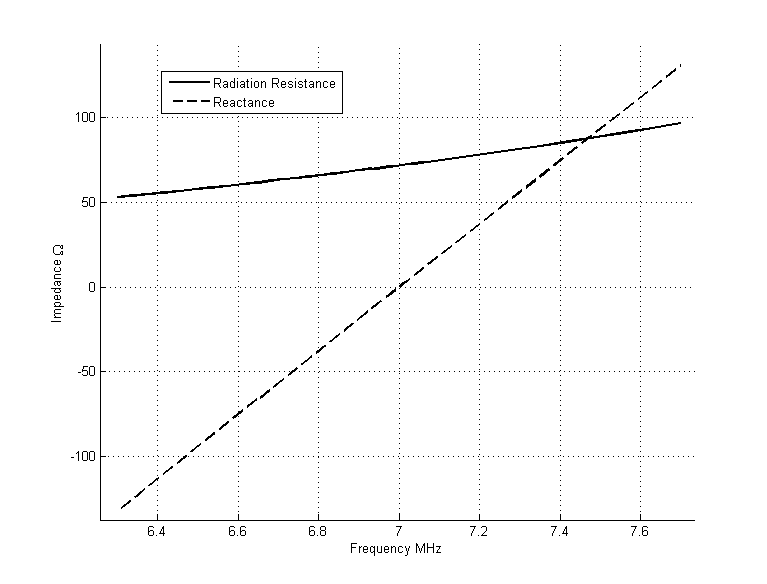
\includegraphics[width=0.45\textwidth]{./img/impf.png}
  \caption{Impedance versus frequency}
  \label{fig:impedance}
\end{figure}
